\documentclass[conference,a4paper]{IEEEtran}
\IEEEoverridecommandlockouts
\usepackage{textcomp}
\usepackage{graphicx}
\usepackage{cite}
\usepackage{algorithm}
\usepackage{algpseudocode}
\usepackage{amsmath}
\usepackage{amssymb}
\usepackage{amsfonts}
\usepackage{color}
\usepackage[tableposition=top]{caption}
\usepackage{setspace}
\usepackage{epstopdf}
\usepackage{graphics}
\usepackage{subfigure}
\usepackage{caption}

\setcounter{secnumdepth}{3}
\setcounter{tocdepth}{3}
\newcounter{lines}
\def \algline { \refstepcounter{lines} \ifthenelse{\value{lines}<10}{0\arabic{lines}:}{\arabic{lines}:} }


\begin{document}
\title{Building the NOMA Simulation Model for Mac Layer Research}

\author{
\authorblockN{\fontsize{11pt}{1em}\selectfont \textbf{PI} XXX  \textbf{CoPI} YYY  \textbf{MTK} \textbf{Contact} ZZZ}\\
\authorblockA{
Ming Jie Yang
}
}
\maketitle

% abstract
%\begin{abstract}
%% describe the project and objectives
The report shows progress on the project that explores non-orthogonal
multiple access (NOMA) with successive interference cancellation (SIC).
The short term objective of current phase is to build a simulation
framework and examine the performance gain with SIC technique. The
system is extended based on LTE architecture.

% brief the content in this report

% brief some result


%\end{abstract}

\section{Status quo}
\label{sec_status_quo}

Briefly, by the previous effort in literature survey, we summarize related 
work as follows.
Some studies investigate non-orthogonal multiple access (NOMA) by theoretical 
models, which are extended from shannon capacity model.
Based on theoretical models, the rule that the optimal order for SIC decoding 
is same as the increasing order of $\frac{|h|^2}{N}$. 
A NOMA/Multiple-Input Multiple-Output (MIMO) scheme is proposed to achieve 
further capacity gain.
Throughput balance of the cell-edge and interior users by using SIC in the 
cellular downlink.
%
% Ideal model above
%

Other works show SIC performance of simulations with respect to physical layer 
design has significant diffrence compared to the theoretical model.
To proceed with research in MAC-layer, a working simulation model based on
existing techniques are built to capture the practical performace trad-off
in NOMA.

\section{Key new insight}
\label{sec_key_new_insight}

1) In Fig.~\ref{fig_alphaVSber}, error propagation in existing 
NOMA PHY techniques (SIC) due to successive decoding of multiplexed 
signals needs to be taken into consideration in the simulation model.
As In the theoretical model, the data of previous stages can be 
fully decoded regarless of the power allocation.
2) The impact of modulation/coding scheme (MCS) selection as
well as the power allocation factor (PAF) among NOMA users
(users that share the same resource block) also needs to be taken
into consideration in the simulation model.
3) For a two-user NOMA system, pairing of users for sharing each
resource block should ensure that the bit error rates (BERs)
achieved at each user are within the tolerable range when the sum
rate is being maximized.

\begin{figure}[t]
\begin{center}
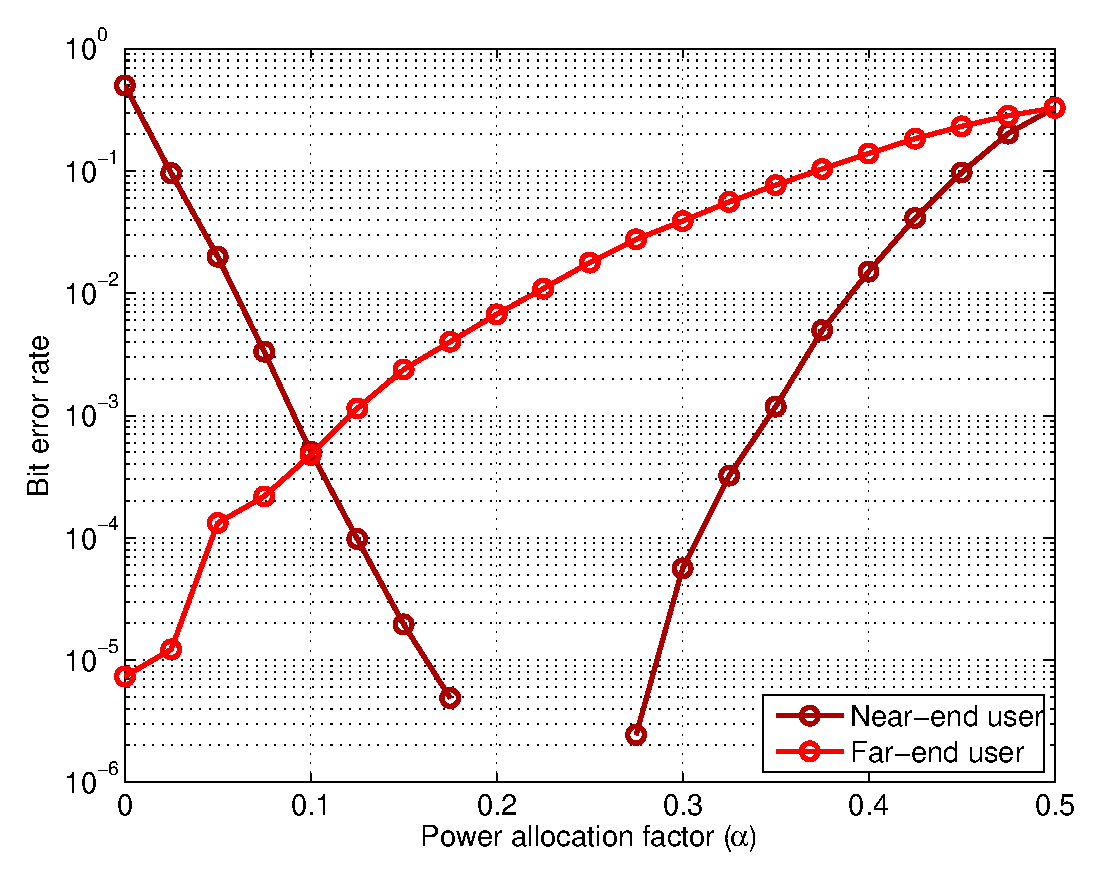
\includegraphics[width=0.9\columnwidth ,angle=0]{figure/alphaVSber.eps}
\caption{BER for different power allocation factor}
\label{fig_alphaVSber}
\end{center}
\end{figure}


\section{Main achievement}
\label{sec_main_achievement}
We have built a physical-layer simulation platform for single-
antenna NOMA with consideration of modulation, channel coding,
and multipath channels based on SIC.
We have obtained the desired MCS/BER model for two-user
NOMA in the two-stage decoding scheme.
We have investigated a simple scheduling algorithm for pairing
users in each OFDM resource block such that the BERs of all
users can satisfy the desired constraint.


\section{How it works}
\label{sec_how_it_works}

\begin{figure}[t]
\begin{center}
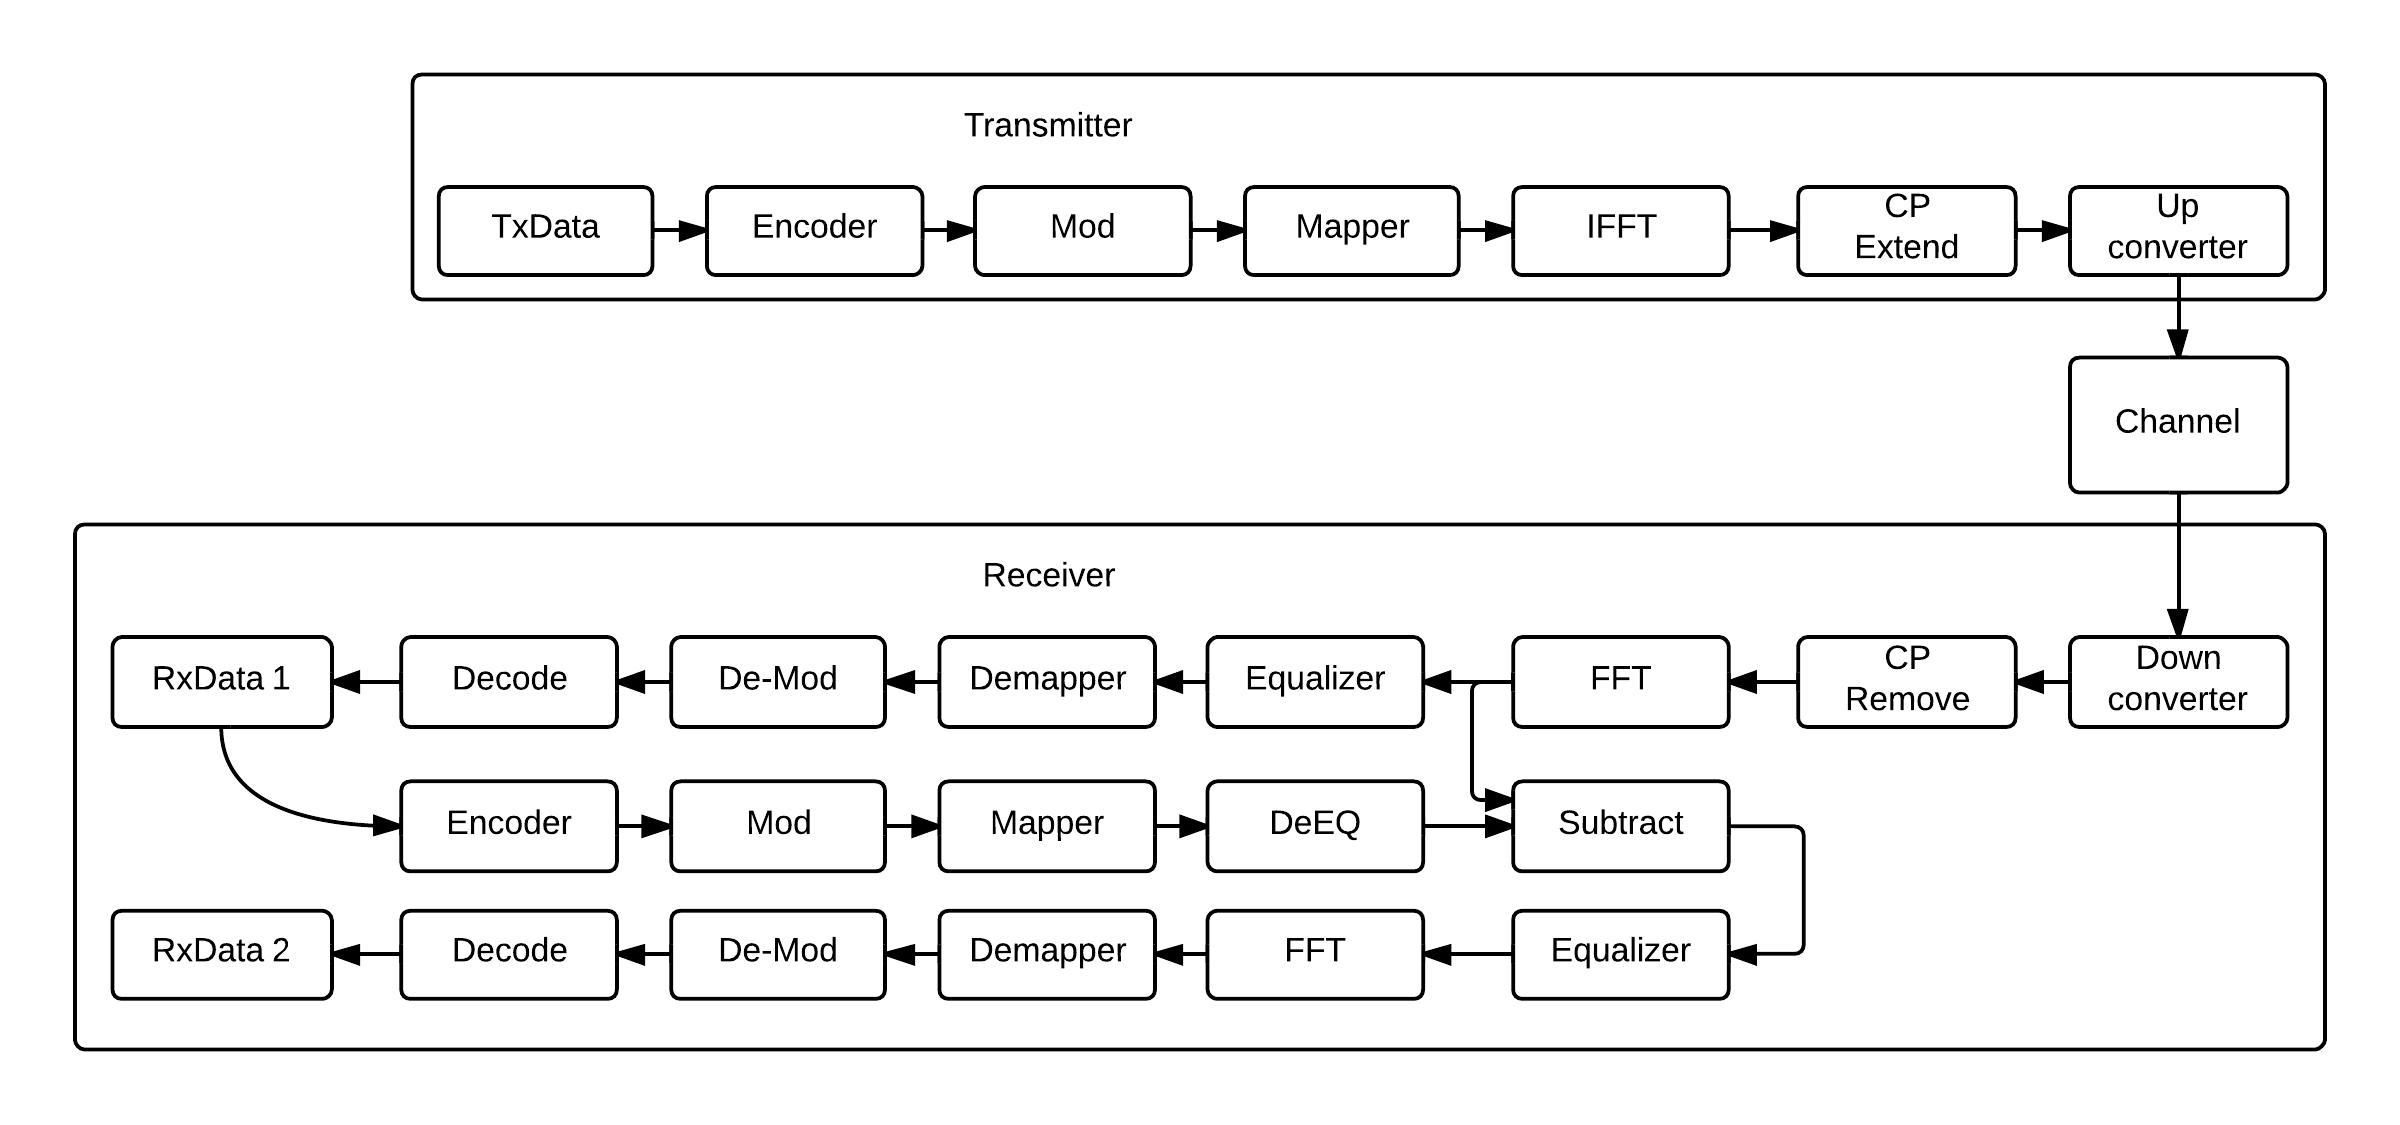
\includegraphics[width=1.0\columnwidth ,angle=0]{figure/systemArch.png}
\caption{simulation architecture}
\label{fig_sys_arch}
\end{center}
\end{figure}

The physical layer simulation is constructed by the system architecture 
shown in Fig.~\ref{fig_sys_arch}.
In this system, the receiver can only extract two layers of multiplexed data.

The system architecture is build with following functional blocks. 1)TxData 
generator: generates binary random bits for transmission, 2)Encoder: encode 
the data by convolutional coding method, 3)Modulator: modulates bits into
symbols, 4)IFFT: maps the frequency domain signals to time domain samples,
5)Cyclic Prefix: appending cyclic prefix, 6)Channel: implement white noise
and multipath enviornments, 7)Equalizer: to compensate the effect of channel.

Fig.~\ref{fig_pair_mcs} shows the highest order of MCS that the users can
achieve in given BER constraint for different channel condition (note that
axis has minus sign.) Here the BER constraint is set to be $10^{-4}$.

To provide quality service in wireless multiple access
network, it’s essential to make proper scheduling between users
when the resources is limited.
Fig.~\ref{fig_my_schedule} shows the topology of
12 users are randomly scattered in 2800 square meter plane.
Each user has to transmit at least once and we have to schedule all users 
in 6 resource blocks with 2 users in each with no overlapping.
Fig.~\ref{fig_my_schedule} shows the schedule result by algorithm~\ref{alg_my}
Pairs of users are painted with different color.

{
\begin{algorithm}[t]
\setcounter{lines}{0}

\algline \textbf{Input}: a set of user equipments, i.e. $\mathbf{V}$

\algline \textbf{Initial}: $CS \leftarrow \varnothing$ \textbackslash\textbackslash schedule set

\algline Sort UEs by its pathloss increasingly.

\textbf{\quad{}\quad{}}$\mathbf{V'} = \{[v_1\medspace v_2 ... v_n] | PL(v_i) \leq PL(v_j) \forall i < j\}$

\algline \textbf{While } $\mathbf{V'}$ is not empty

\algline \textbf{\quad{}} $u = \mathbf{V'}.first()$ \textbackslash\textbackslash select the first element

\algline \textbf{\quad{}For } $r \in \mathbf{V'},\medspace r\neq u$

\algline \textbf{\quad{}}\textbf{\quad{}If } $pair(u,\medspace r)$ is feasible for given constraint

\algline \textbf{\quad{}}\textbf{\quad{}}\textbf{\quad{}} $\mathbf{M} =pair(u,\medspace r).getMCS()$ \textbackslash\textbackslash feasible MCSs

\algline \textbf{\quad{}}\textbf{\quad{}}\textbf{\quad{}For } $W_{m}, m\in \textbf{M}$

\algline \textbf{\quad{}}\textbf{\quad{}}\textbf{\quad{}}\textbf{\quad{}If } $W_{m} > best$

\algline \textbf{\quad{}}\textbf{\quad{}}\textbf{\quad{}}\textbf{\quad{}}\textbf{\quad{}} $best \leftarrow W_{m}$

\algline \textbf{\quad{}}\textbf{\quad{}}\textbf{\quad{}}\textbf{\quad{}}\textbf{\quad{}} $r' \leftarrow r$

\algline \textbf{\quad{}}\textbf{\quad{}}\textbf{\quad{}}\textbf{\quad{}End If}

\algline \textbf{\quad{}}\textbf{\quad{}}\textbf{\quad{}End For}

\algline \textbf{\quad{}}\textbf{\quad{}End If}

\algline \textbf{\quad{}End For}

\algline \textbf{\quad{}If } $v'$ exists \textbackslash\textbackslash $u$ can form a pair.

\algline \textbf{\quad{}}\textbf{\quad{}} $\mathbf{V'}\leftarrow \mathbf{V'}\backslash \{r', u\}$, $CS \leftarrow CS \bigcup \{r', u\}$

\algline \textbf{\quad{}Else }

\algline \textbf{\quad{}}\textbf{\quad{}} $\mathbf{V'}\leftarrow \mathbf{V'}\backslash \{u\}$, $CS \leftarrow CS \bigcup \{u\}$

\algline \textbf{\quad{}End If }

\algline \textbf{End While}

\algline \textbf{Return} $best,\medspace CS$

\caption{\label{alg_my} Scheduling transmission pairs iteratively}
\end{algorithm}
}

\begin{figure}[t]
\begin{center}
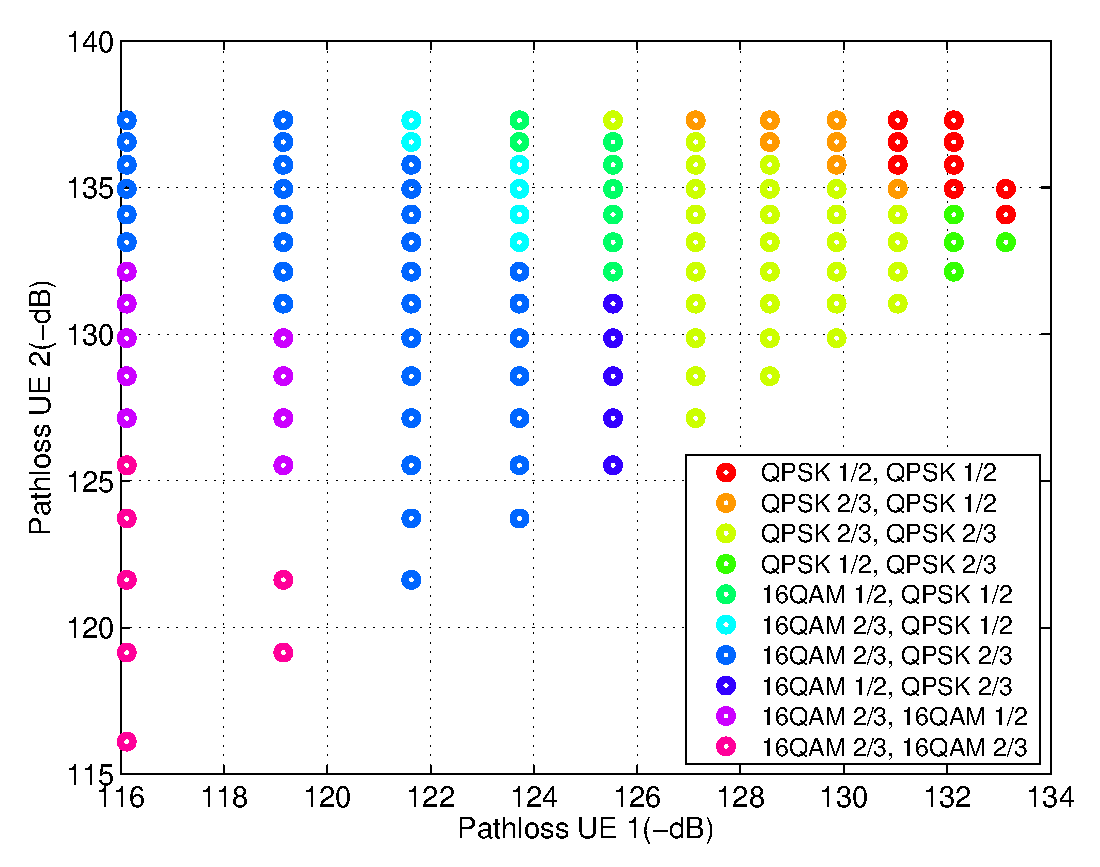
\includegraphics[width=0.9\columnwidth ,angle=0]{figure/pair_mcs.eps}
\caption{MCS supported for BER constraint $10^{-4}$}
\label{fig_pair_mcs}
\end{center}
\end{figure}

\begin{figure}[t]
\begin{center}
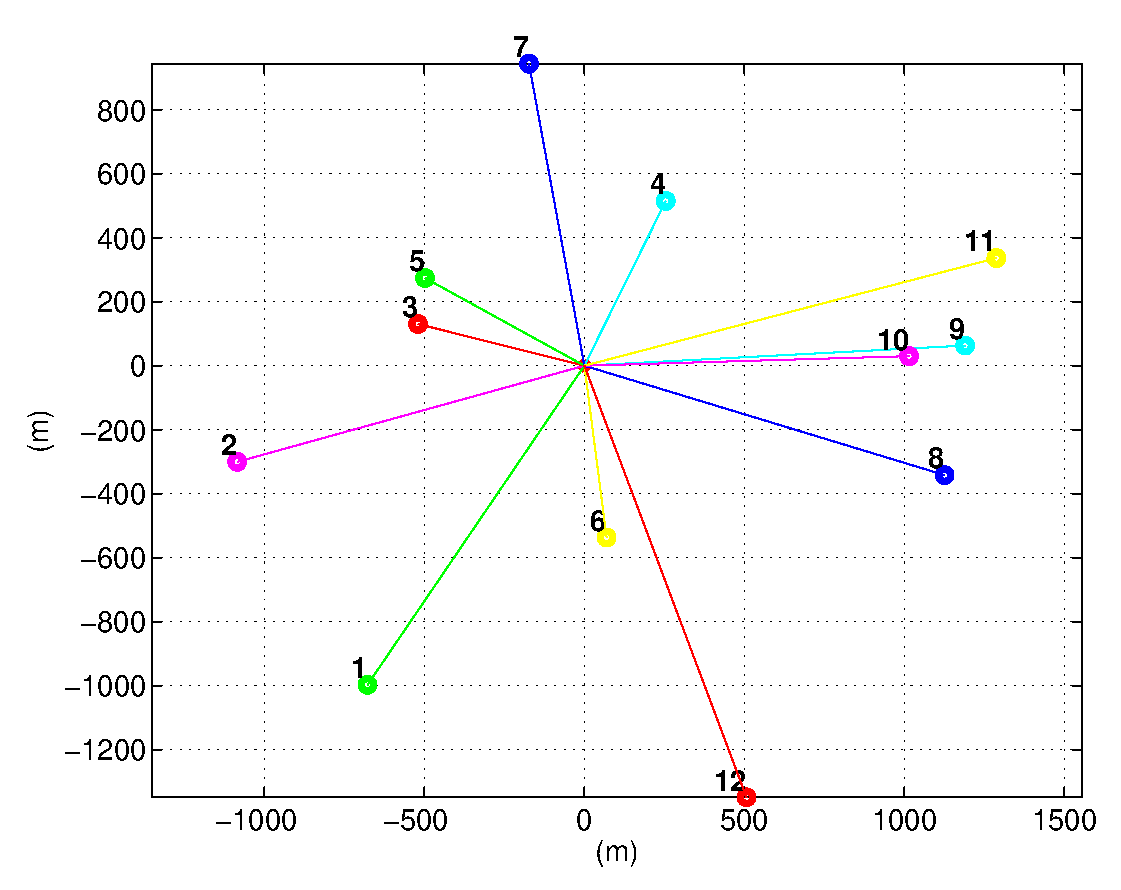
\includegraphics[width=0.9\columnwidth ,angle=0]{figure/my_schedule.eps}
\caption{Scheduled transmission pairs by Alg. 1}
\label{fig_my_schedule}
\end{center}
\end{figure}

%\begin{figure}[t]
%  \centering
%  \subfigure[random caption 1]{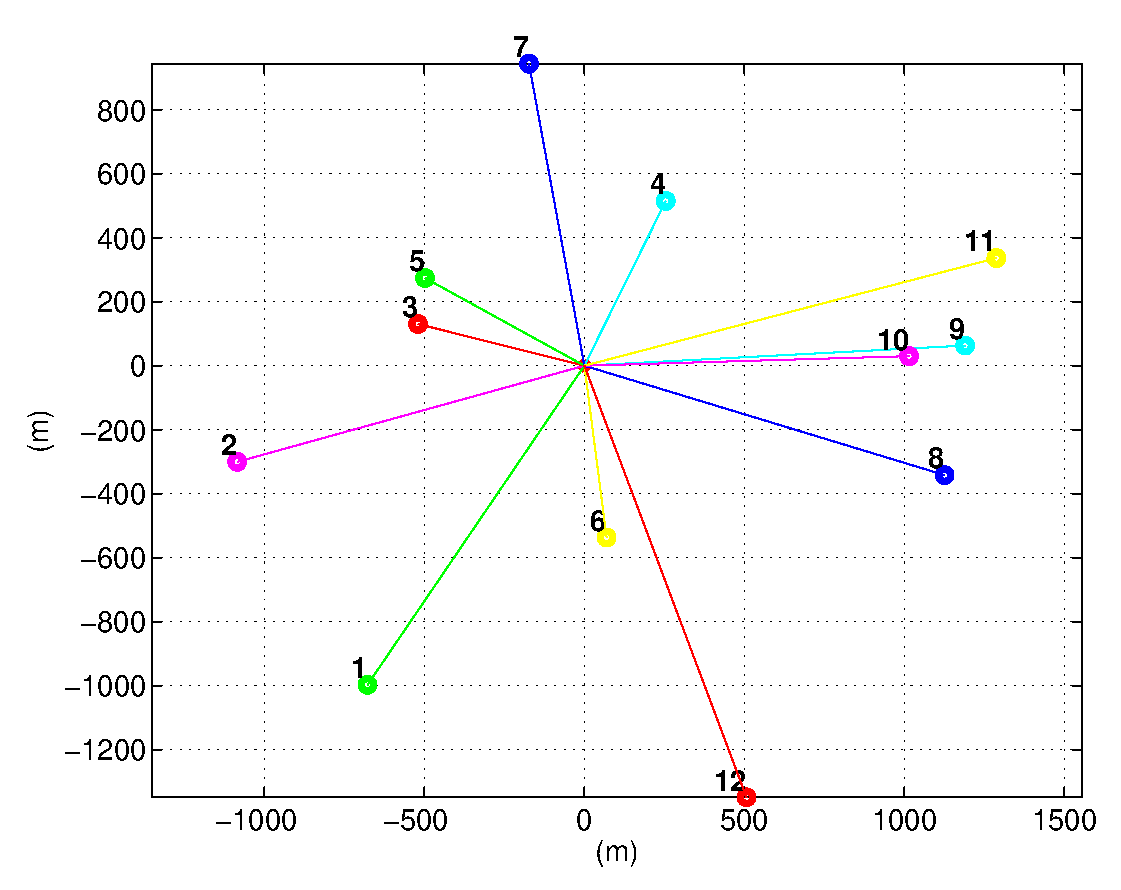
\includegraphics[width=0.45\columnwidth]{figure/my_schedule.eps}}\quad
%  \subfigure[random caption 2]{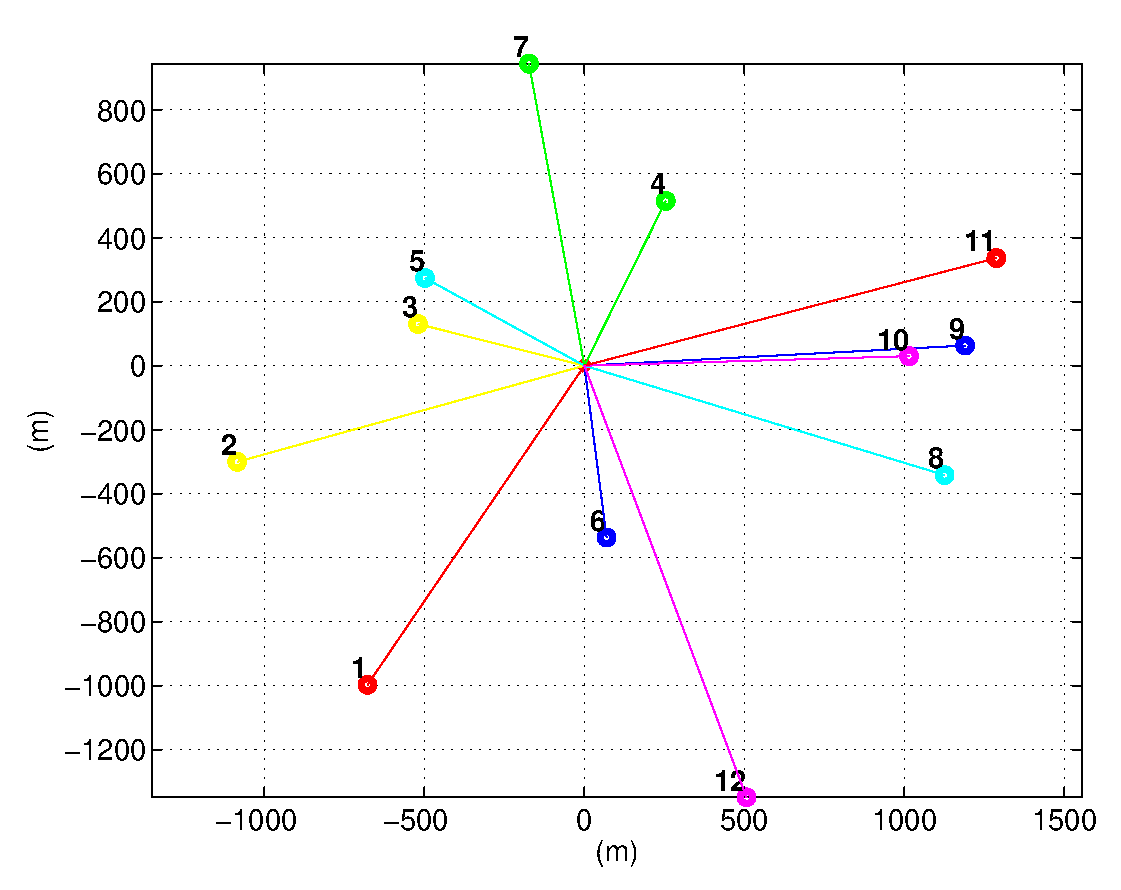
\includegraphics[width=0.45\columnwidth]{figure/schedule_result.eps}}
%\caption{caption}
%\end{figure}


\section{Risk limitation and assumptions}
\label{sec_risk_limit}
The base station transmit multiplexed signal from two independent sources.
The receiver is aware of number of multiplexed user data and thus no further
detection is needed to identify the depth of decoding order.
Full channel state condition is assume in the simulation, no channel estimation
or receiver manufacture defect is taken into consideration.
As an investigation of the limitation of NOMA with SIC, the BS can only transmit
signals of two sources utmost.

\section{Quantitative impact}
\label{sec_impact}
We have found that a 20\% performance gain in the (weighted) sum
rate can be achieved when the paired users have a path-loss ratio
of 10. The performance gain increases as the difference in the
channel condition (path loss) keeps increasing.
Best MCS for two-user NOMA based on the obtained MCS/BER model 
for two-user NOMA (right figure), the proposed scheduling algorithm 
can pair users with 91.67\% optimality (for a 12-user downlink scenario)
without incurring the complexity needed in exhaustive search.


\section{End goals}
\label{sec_end_goals}
Based on the NOMA simulation model and the two-user
scheduling algorithm that we have completed so far, our goal in
the future is to explore more generic problems and algorithms
for resource allocation, scheduling, and power control at the
MAC layer for optimizing the performance of NOMA under the
desirable computation complexity and communication overheads.
The simulation model for single-antenna NOMA will be extended to
MIMO such that clustered-based resource allocation and
scheduling can be investigated in the future.


%\section{Conclusion}
%\label{sec_conclusion}

%After surveying papers, we figure out that the NOMA with SIC has a little difference in their analysis. For DOCOMO, the capacity is simply represented by ideal interference cancellation as (\ref{eq_sic_shannon}). For Bell Lab, they take the modulation and PER into consideration and the simulation results show that capacity is lower than the analysis of DOCOMO. They also propose some algorithms about resource allocation and schedule by optimization algorithm and S4 algorithm.

\section{Plan for the Next Month}
\label{sec_futureWork}

In the next month, we plan to continue investigation of NOMA on physical and MAC layers to better 
equip ourselves with state-of-the-art research advances on NOMA. In addition to theoretic, ideal models
for NOMA, we also plan to investigate more closely the simulation models presented in~\cite{cite_bell1} to lay a
more solid ground for
the resource allocation and scheduling techniques to be investigated in this project.

%In the following months, we will start to analyze NOMA with SIC and create the SNR-modulation model. What's more, in order to let optimization conveniently, we will also construct an approximation equation named SNR-throughput equation to fit the model. After finishing SNR-modulation model and SNR-throughput equation, we will propose algorithms managing resource allocation and schedule and present our results by simulation. Therefore, the SNR-modulation model, SNR-throughput equation, and algorithms will jointly construct into first version's simulator. 

%\section{Research Byproduct}
%\label{sec_product}

%None.


% citations
%\bibliographystyle{IEEEtran}
%\bibliography{cite}

\end{document}
